% +------------------------------------------------------------------------+
% | Reference manual page: HalfedgeDS_decorator.tex
% +------------------------------------------------------------------------+
% | 22.03.1999   Lutz Kettner
% | Package: HalfedgeDS
% |
\RCSdef{\RCSHalfedgeDSdecoratorRev}{$Id$}
\RCSdefDate{\RCSHalfedgeDSdecoratorDate}{$Date$}
% +------------------------------------------------------------------------+

\ccRefPageBegin

%%RefPage: end of header, begin of main body
% +------------------------------------------------------------------------+


\begin{ccRefClass}{HalfedgeDS_decorator<HDS>}

\ccDefinition

The classes \ccc{CGAL::HalfedgeDS_items_decorator<HDS>},
\ccc{CGAL::HalfedgeDS_decorator<HDS>}, and
\ccc{CGAL::HalfedgeDS_const_decorator<HDS>} provide additional functions
to examine and to modify a halfedge data structure \ccc{HDS}. The class
\ccc{CGAL::HalfedgeDS_items_decorator<HDS>} provides additional functions
for vertices, halfedges, and faces of a halfedge data structure
without knowing the containing halfedge data structure. The class
\ccc{CGAL::HalfedgeDS_decorator<HDS>} stores a reference to the halfedge
data structure and provides functions that modify the halfedge data
structure, for example Euler-operators. The class
\ccc{CGAL::HalfedgeDS_const_decorator<HDS>} stores a const reference to
the halfedge data structure. It contains non-modifying functions, for
example the test for validness of the data structure.

All these additional functions take care of the different capabilities
a halfedge data structure may have or may not have.  The functions
evaluate the type tags of the halfedge data structure to decide on the
actions. If a particular feature is not supported nothing is done.
Note that for example the creation of new halfedges is mandatory for
all halfedge data structures and will not appear here again.

\ccInclude{CGAL/HalfedgeDS_decorator.h}

\ccInheritsFrom

\ccRefIdfierPage{CGAL::HalfedgeDS_items_decorator<HDS>}

\ccCreation
\ccCreationVariable{D}

\ccThree{Halfedge_handle}{D.set_new_vertexA( Halfe h, Point p);;;}{}
\ccThreeToTwo

\ccTagFullDeclarations
\ccConstructor{HalfedgeDS_decorator( HDS& hds);}
    {keeps internally a reference to \ccc{hds}.}
\ccTagDefaults

% -----------------------------------------
\ccHeading{Creation of New Items}

\ccMethod{Vertex_handle vertices_push_back( const Vertex& v);}{
    appends a copy of $v$ to \ccc{hds} if vertices are supported.
    Returns a handle of the new vertex, or \ccc{Vertex_handle()} otherwise.}
\ccGlue
\ccMethod{Face_handle faces_push_back( const Face& f);}{
    appends a copy of $f$ to \ccc{hds} if faces are supported.
    Returns a handle of the new face, or \ccc{Face_handle()} otherwise.}

% -----------------------------------------
\ccHeading{Creation of New Composed Items}

\ccMethod{Halfedge_handle create_loop();}{
    returns handle of a halfedge from a newly created loop in \ccc{hds}
    consisting of a single closed edge, one vertex and two faces (if
    supported respectively).}
\ccGlue
\ccMethod{Halfedge_handle create_segment();}{
    returns a halfedge from a newly created segment in \ccc{hds}
    consisting of a single open edge, two vertices and one face (if
    supported respectively).}

% -----------------------------------------
\ccHeading{Removal of Elements}

\ccThree{void}{D.vertices_erase( Vertex_handle v);}{}

The following member functions do {\em not\/} update affected
incidence relations except if mentioned otherwise.

\ccMethod{void vertices_pop_front();}{
    removes the first vertex if vertices are supported.
    \ccCommentHeading{Requirement} \ccc{Supports_removal} $\equiv$
    \ccc{CGAL::Tag_true}.}
\ccGlue
\ccMethod{void vertices_pop_back();}{
    removes the last vertex if vertices are supported.}
\ccGlue
\ccMethod{void vertices_erase( Vertex_handle v);}{
    removes the vertex $v$ if vertices are supported.
    \ccCommentHeading{Requirement} \ccc{Supports_removal} $\equiv$
    \ccc{CGAL::Tag_true}.}
\ccGlue
\ccMethod{void vertices_erase( Vertex_handle first, Vertex_handle last);}{
    removes the range $[\ccc{first},\ccc{last})$ if vertices
    are supported. \ccCommentHeading{Requirement} \ccc{Supports_removal}
    $\equiv$ \ccc{CGAL::Tag_true}.}

\ccMethod{void faces_pop_front();}{
    removes the first face if faces are supported.
    \ccCommentHeading{Requirement} \ccc{Supports_removal} $\equiv$
    \ccc{CGAL::Tag_true}.}
\ccGlue
\ccMethod{void faces_pop_back();}{
    removes the last face if faces are supported.}
\ccGlue
\ccMethod{void faces_erase( Face_handle f);}{
    removes the face $f$ if faces are supported.
    \ccCommentHeading{Requirement} \ccc{Supports_removal} $\equiv$
    \ccc{CGAL::Tag_true}.}
\ccGlue
\ccMethod{void faces_erase( Face_handle first, Face_handle last);}{
    removes the range $[\ccc{first},\ccc{last})$ if faces are
    supported. \ccCommentHeading{Requirement} \ccc{Supports_removal}
    $\equiv$ \ccc{CGAL::Tag_true}.}

\ccMethod{void erase_face( Halfedge_handle h);} {removes the
   face incident to \ccc{h} from \ccc{hds} and changes all halfedges
   incident to the face into border edges or removes them from the
   halfedge data structure if they were already border edges. If this
   creates isolated vertices they get removed as well. See
   \ccc{make_hole(h)} for a more specialized variant.
   \ccPrecond \ccc{h->is_border() == false}.
   \ccCommentHeading{Requirement} If faces are supported,
   \ccc{Supports_removal} $\equiv$ \ccc{CGAL::Tag_true}.}

\ccMethod{void erase_connected_component( Halfedge_handle h);}
    {removes the  vertices, halfedges, and faces that belong to the
     connected component of $h$. \ccPrecond For all halfedges $g$ in the
     connected component \ccc{g.next() != Halfedge_handle()}.
     \ccCommentHeading{Requirement}  \ccc{Supports_removal} $\equiv$
     \ccc{CGAL::Tag_true}.}

\ccMethod{unsigned int keep_largest_connected_components(unsigned int nb_components_to_keep);}
    {Erases the small connected components and the isolated vertices.
     Keep \ccc{nb_components_to_keep} largest connected components.
     Returns the number of connected components erased (ignoring isolated vertices).
     \ccCommentHeading{Requirement} supports vertices, halfedges, and removal operation.}

% -----------------------------------------
\ccHeading{Modifying Functions (For Border Halfedges)}

\ccThree{Halfedge_handle}{hds.split_f}{}

\ccMethod{void make_hole( Halfedge_handle h);}
   {removes the face incident to \ccc{h} from \ccc{hds} and creates a hole.
    \ccPrecond \ccc{h != Halfedge_handle()} and \ccc{!(h->is_border())}.
    \ccCommentHeading{Requirement} If faces are supported,
    \ccc{Supports_removal} $\equiv$ \ccc{CGAL::Tag_true}.}

\ccMethod{Halfedge_handle fill_hole( Halfedge_handle h);}
   {fills the hole incident to \ccc{h} with a new face from \ccc{hds}.
    Returns \ccc{h}.
    \ccPrecond \ccc{h != Halfedge_handle()} and \ccc{h->is_border()}.}

\ccMethod{Halfedge_handle fill_hole( Halfedge_handle h, const Face& f);}
   {fills the hole incident to \ccc{h} with a copy of face $f$.
    Returns \ccc{h}.
    \ccPrecond \ccc{h != Halfedge_handle()} and \ccc{h->is_border()}.}

\ccMethod{Halfedge_handle add_face_to_border( Halfedge_handle h,
                                              Halfedge_handle g);}
   {extends the surface with a new face from \ccc{hds} into the hole
    incident to $h$ and $g$. It creates a new edge connecting the vertex
    denoted by $g$ with the vertex denoted by $h$ and fills this separated
    part of the hole with a new face, such that the new face is incident
    to $g$. Returns the new halfedge that is incident to the new face.
    \ccPrecond \ccc{h != Halfedge_handle()}, \ccc{g != Halfedge_handle()},
    \ccc{h->is_border()}, \ccc{g->is_border()} and $g$ can be reached
    along the hole starting with $h$.}

\ccMethod{Halfedge_handle add_face_to_border( Halfedge_handle h,
                                              Halfedge_handle g,
                                              const Face& f);}
   {extends the surface with a copy of face $f$ into the hole
    incident to $h$ and $g$. It creates a new edge connecting the tip of
    $g$ with the tip of $h$ and fills this separated part of the hole with a
    copy of face $f$, such that the new face is incident to $g$. Returns
    the new halfedge that is incident to the new face.
    \ccPrecond \ccc{h != Halfedge_handle()}, \ccc{g != Halfedge_handle()},
    \ccc{h->is_border()}, \ccc{g->is_border()} and $g$ can be reached
    along the hole starting with $h$.}

% -----------------------------------------
\ccHeading{Modifying Functions (Euler Operators)}

\ccThree{Halfedge_handle}{hds.split_f}{}

The following Euler operations modify consistently the combinatorial
structure of the halfedge data structure. The geometry remains unchanged.
Note that well known graph operations are also captured with these
Euler operators, for example an edge contraction is equal to a
\ccc{join_vertex()} operation, or an edge removal to \ccc{join_face()}.

Given a halfedge data structure \ccc{hds} and a halfedge handle $h$
four special applications of the Euler operators are worth mentioning:
\ccc{split_vertex(h,h)} results in an antenna emanating from the tip
of \ccc{h}; \ccc{split_vertex(h,h->next()->opposite())} results in an edge
split of the halfedge \ccc{h->next} with a new vertex in-between;
\ccc{split_face(h,h)} results in a loop directly following \ccc{h};
and \ccc{split_face(h,h->next())} results in a bridge parallel to
the halfedge \ccc{h->next} with a new face in-between.

\begin{ccTexOnly}
    \begin{center}
      \parbox{\textwidth}{%
          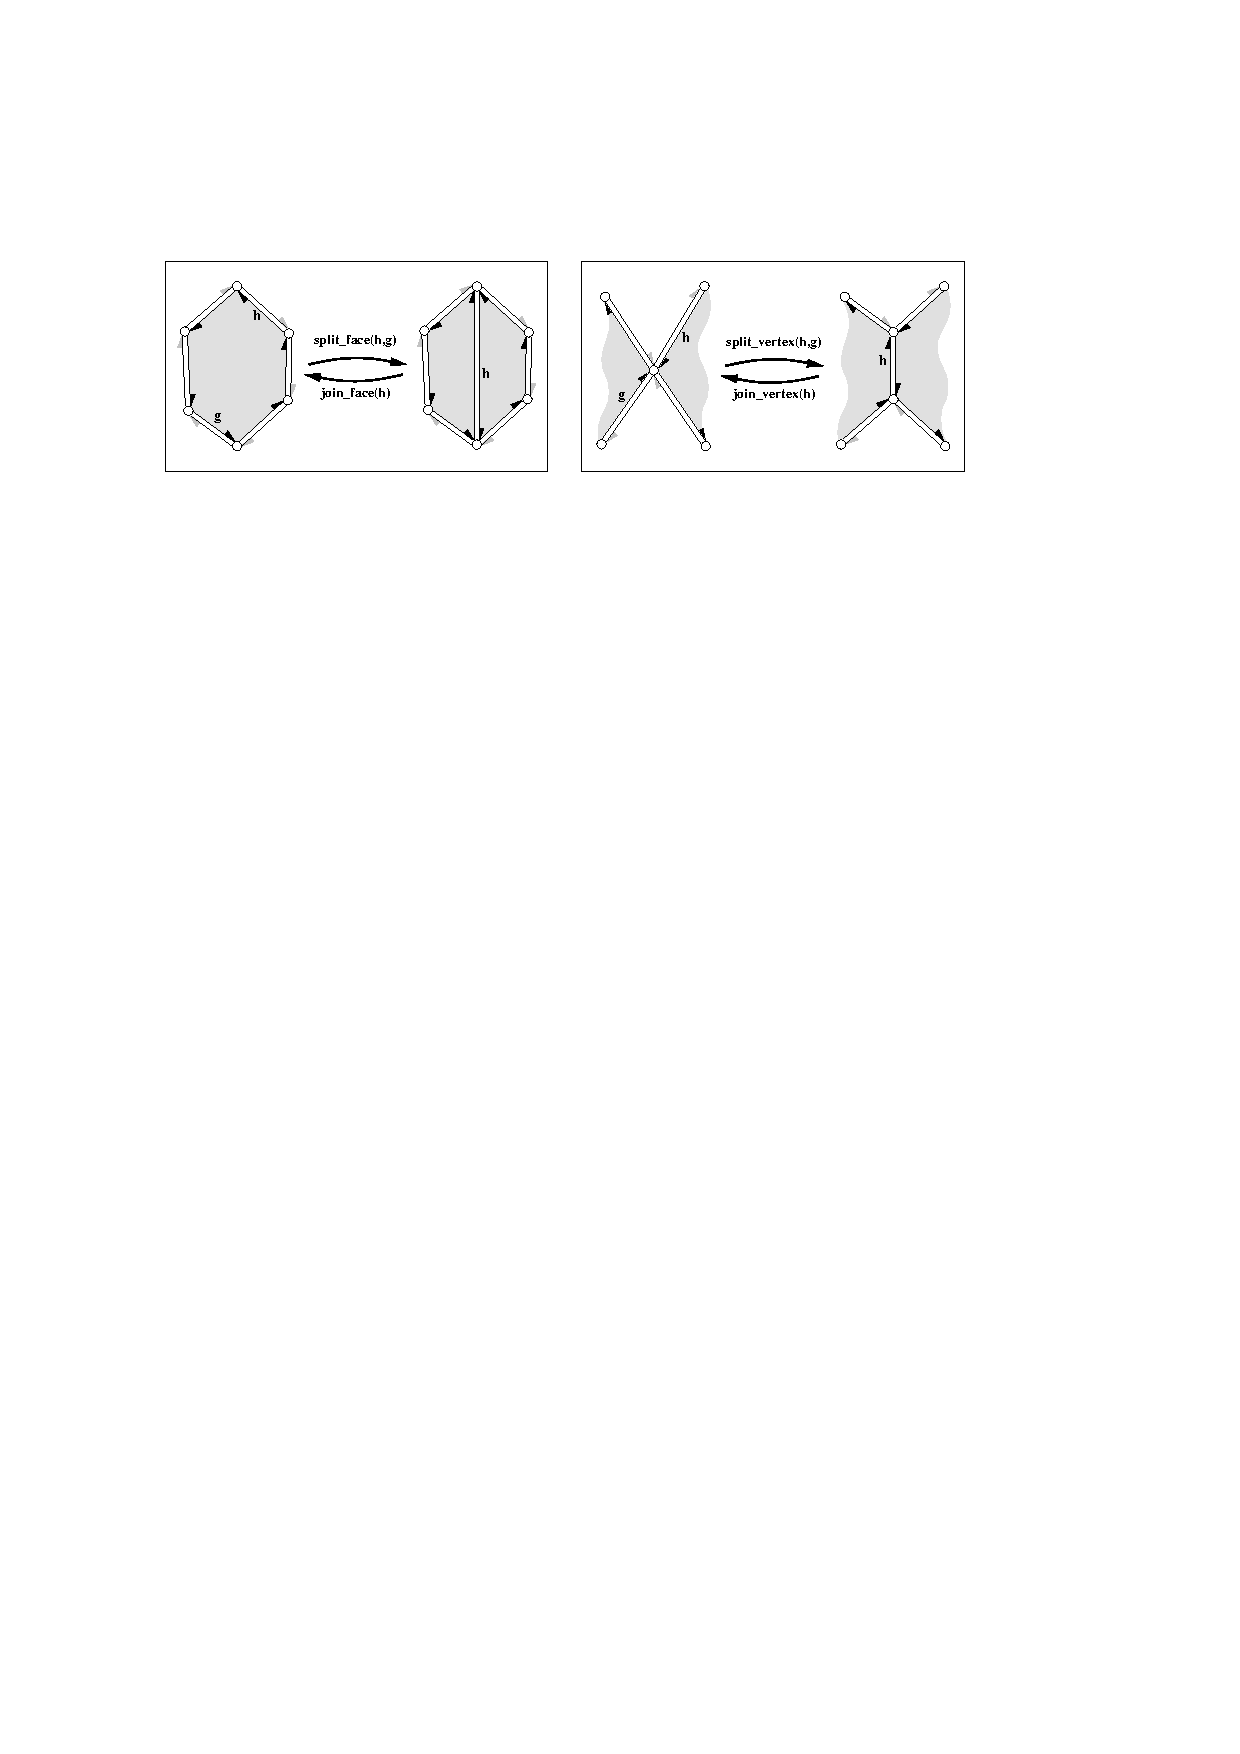
\includegraphics[width=\textwidth]{HalfedgeDS_ref/fig/euler_hds}%
      }
    \end{center}
\end{ccTexOnly}

\begin{ccHtmlOnly}
    <CENTER>
    <img src="fig/euler_face.gif" alt="Euler Operator: Face"><P>
    </CENTER>
\end{ccHtmlOnly}

\ccMethod{Halfedge_handle split_face( Halfedge_handle h, Halfedge_handle g);}
    {splits the face incident to \ccc{h} and \ccc{g} into two faces
     with a new diagonal between the two vertices denoted by \ccc{h} and
     \ccc{g} respectively. The second (new) face obtained from
     \ccc{hds} is a copy of the first face. Returns \ccc{h->next()} after the
     operation, i.e., the new diagonal. The new face is to the right of the
     new diagonal, the old face is to the left. The time is proportional
     to the distance from \ccc{h} to \ccc{g} around the face.}

\ccMethod{Halfedge_handle join_face( Halfedge_handle h);}
    {joins the two faces incident to $h$. The face incident to
      \ccc{h->opposite()} gets removed from \ccc{hds}. Both faces might be
    holes. Returns the predecessor of $h$ around the face. The invariant
    \ccc{join_face( split_face( h, g))} returns $h$ and keeps
    the data structure unchanged. The time is proportional to the size
    of the face removed and the time to compute \ccc{h->prev()}.
    \ccCommentHeading{Requirement} \ccc{Supports_removal} $\equiv$
    \ccc{CGAL::Tag_true}.}


\begin{ccHtmlOnly}
    <CENTER>
    <img src="fig/euler_vertex.gif" alt="Euler Operator: Vertex"><P>
    </CENTER>
\end{ccHtmlOnly}

\ccMethod{Halfedge_handle split_vertex( Halfedge_handle h, Halfedge_handle g);}
    {splits the vertex incident to \ccc{h} and \ccc{g} into two vertices
     and connects them with a new edge. The second (new) vertex
     obtained from \ccc{hds} is a copy of the first vertex. Returns
     \ccc{h->next()->opposite()} after the operation, i.e., the new edge
     in the orientation towards the new vertex. The time is proportional
     to the distance from \ccc{h} to \ccc{g} around the vertex.}

\ccMethod{Halfedge_handle join_vertex( Halfedge_handle h);}
    {joins the two vertices incident to $h$. The vertex denoted by
     \ccc{h->opposite()} gets removed by \ccc{hds}. Returns the predecessor of
     $h$ around the vertex, i.e., \ccc{h->opposite()->prev()}. The invariant
     \ccc{join_vertex( split_vertex( h, g))} returns $h$
     and keeps the polyhedron unchanged.
     The time is proportional to the degree of the vertex removed and
     the time to compute \ccc{h->prev()} and \ccc{h->opposite()->prev()}.
     \ccCommentHeading{Requirement} \ccc{Supports_removal} $\equiv$
     \ccc{CGAL::Tag_true}.}

\begin{ccTexOnly}
    \begin{center}
      \parbox{0.52\textwidth}{%
          \includegraphics[width=0.52\textwidth]%
              {HalfedgeDS_ref/fig/euler_center}%
      }
    \end{center}
\end{ccTexOnly}

\begin{ccHtmlOnly}
    <CENTER>
    <img src="fig/euler_center.gif" alt="Euler Operator: Center Vertex"><P>
    </CENTER>
\end{ccHtmlOnly}

\ccMethod{Halfedge_handle create_center_vertex( Halfedge_handle h);}
    {barycentric triangulation of \ccc{h->face()}. Creates a new vertex,
     a copy of \ccc{h->vertex()}, and connects it to each vertex incident
     to \ccc{h->face()} splitting \ccc{h->face()} into triangles.
     \ccc{h} remains incident to the original face, all other triangles
     are copies of this face. Returns the halfedge \ccc{h->next()}
     after the operation, i.e., a halfedge pointing to the new vertex.
     The time is proportional to the size of the face.
     \ccPrecond \ccc{h} is not a border halfedge.}

\ccMethod{Halfedge_handle erase_center_vertex( Halfedge_handle g);}
    {reverses \ccc{create_center_vertex}. Erases the
     vertex pointed to by \ccc{g} and all incident halfedges thereby
     merging all incident faces. Only \ccc{g->face()} remains.
     The neighborhood of \ccc{g->vertex()} may not be triangulated,
     it can have larger faces. Returns the halfedge \ccc{g->prev()}.
     Thus, the invariant \ccc{h == erase_center_vertex(
     create_center_vertex(h))} holds if \ccc{h} is not a border halfedge.
     The time is proportional to the sum of the size of all incident faces.
     \ccPrecond None of the incident faces of \ccc{g->vertex()} is
     a hole. There are at least two distinct faces incident
     to the faces that are incident to \ccc{g->vertex()}. (This
     prevents the operation from collapsing a volume into two faces
     glued together with opposite orientations, such as would
     happen with any vertex of a tetrahedron.)
     \ccCommentHeading{Requirement} \ccc{Supports_removal} $\equiv$
     \ccc{CGAL::Tag_true}.}

\newpage

\begin{ccTexOnly}
    \begin{center}
      \parbox{0.636\textwidth}{%
          \includegraphics[width=0.636\textwidth]%
              {HalfedgeDS_ref/fig/euler_loop}%
      }
    \end{center}
\end{ccTexOnly}

\begin{ccHtmlOnly}
    <CENTER>
    <img src="fig/euler_loop.gif" alt="Euler Operator: Loop"><P>
    </CENTER>
\end{ccHtmlOnly}

\ccMethod{Halfedge_handle split_loop( Halfedge_handle h,
                                      Halfedge_handle i,
                                      Halfedge_handle j);}
   {cuts the halfedge data structure into two parts along the cycle $(h,i,j)$.
    Three new vertices (one copy for each vertex in the cycle) and three
    new halfedges (one copy for each halfedge in the cycle), and two new
    triangles are created. $h,i,j$ will be incident to the first new triangle.
    The return value will be the halfedge incident to the second new triangle
    which is the copy of \ccc{h-opposite()}.
    \ccPrecond $h,i,j$ denote distinct, consecutive vertices of the
    halfedge data structure and form a cycle: i.e., \ccc{h->vertex() ==
    i->opposite()->vertex()}, \ldots, \ccc{j->vertex() ==
    h->opposite()->vertex()}.}

\ccMethod{Halfedge_handle join_loop( Halfedge_handle h, Halfedge_handle g);}
   {glues the boundary of the two faces denoted by $h$ and $g$ together
    and returns $h$. Both faces and the vertices along the face denoted
    by $g$ gets removed. Both faces may be holes. The invariant
    \ccc{join_loop( h, split_loop( h, i, j))} returns $h$ and keeps the
    data structure unchanged.
    \ccPrecond The faces denoted by $h$ and $g$ are different and have
    equal degree (i.e., number of edges).
    \ccCommentHeading{Requirement} \ccc{Supports_removal} $\equiv$
    \ccc{CGAL::Tag_true}.}


% -----------------------------------------
\ccHeading{Validness Checks}
\ccThree{Halfe}{dge_handlehds.split_f}{}

These operations are the same as for
\ccc{CGAL::HalfedgeDS_const_decorator<HDS>}.
\begin{ccTexOnly}
    See their documentation on page~\pageref{pageHalfedgeDSconstDecoratorRef}.
\end{ccTexOnly}

\ccMethod{bool is_valid( bool verbose = false, int level = 0) const;}{}

\ccMethod{bool normalized_border_is_valid( bool verbose = false) const;}{}

% -----------------------------------------
\ccHeading{Miscellaneous}

\ccMethod{void   inside_out();}
    {reverses face orientations. \ccPrecond \ccc{is_valid()} of level three.}


% -----------------------------------------
\ccSeeAlso

\ccRefIdfierPage{CGAL::HalfedgeDS_items_decorator<HDS>}\\
\ccRefIdfierPage{CGAL::HalfedgeDS_const_decorator<HDS>}

% -----------------------------------------
\ccExample

The following program fragment illustrates the implementation of the
Euler operator \ccc{split_vertex()} for a simplified polyhedron class.

\begin{ccExampleCode}
template <class Traits>
namespace CGAL {
    class Polyhedron {
        typedef HalfedgeDS_default<Traits> HDS;
        HDS hds;
    public:
        // ...
        Halfedge_handle split_vertex( Halfedge_handle h, Halfedge_handle g) {
            HalfedgeDS_decorator<HDS> D(hds);
            // Stricter preconditions than for HalfedgeDS only.
            CGAL_precondition( D.get_vertex(h) == D.get_vertex(g));
            CGAL_precondition( h != g);
            return D.split_vertex( h, g);
        }
    };
}
\end{ccExampleCode}

\end{ccRefClass}

% +------------------------------------------------------------------------+
%%RefPage: end of main body, begin of footer
\ccRefPageEnd
% EOF
% +------------------------------------------------------------------------+

